%************************************************
\chapter{Introduccion}\label{ch:introduction}
%************************************************

En la primer sección de este capítulo se explican los motivos que llevan al desarrollo de este trabajo, mientras que en la segunda sección se detallan los principales objetivos buscados. 
Por último se incluye también una breve descripción de la manera en que está organizada la tesis.

\section{Motivación}
La obtención de modelos tridimensionales precisos y de alta calidad es crucial para un amplio rango de aplicaciones, entre las que se puede nombrar el control de robots inteligentes, la detección de obstáculos para vehículos automáticos, el control de calidad, la ingeniería inversa, entre muchas otras \cite{chen2000overview}. En la industria existe la necesidad de medir con precisión la geometría de diversos objetos para acelerar el desarrollo de productos y asegurar la calidad del proceso de manufactura. Mediante el relevamiento de la geometría de objetos se pueden automatizar tareas como la inspección y el reconocimiento de defectos en la línea de producción.

\begin{figure}[!bth]
    \myfloatalign
        \subfloat[Control dimensional en la industria automotriz]
        {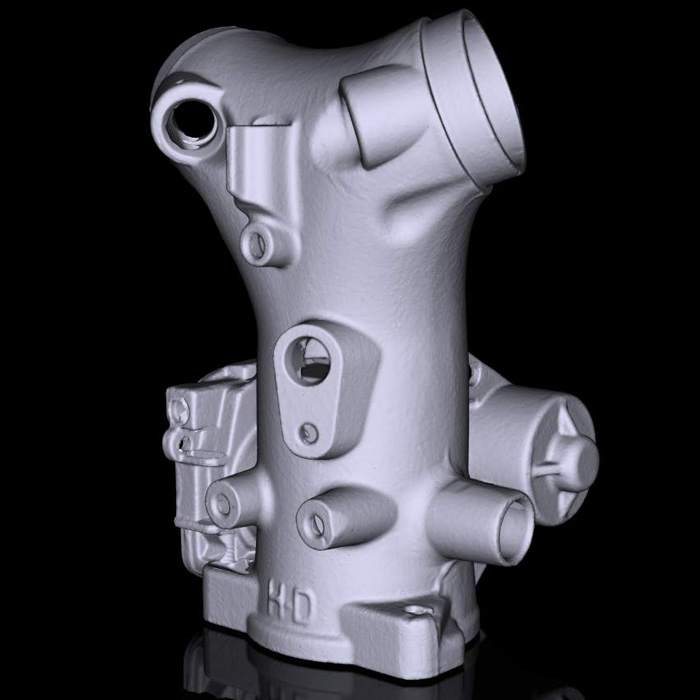
\includegraphics[width=0.49\linewidth]{images/lmi3d/throttle}
         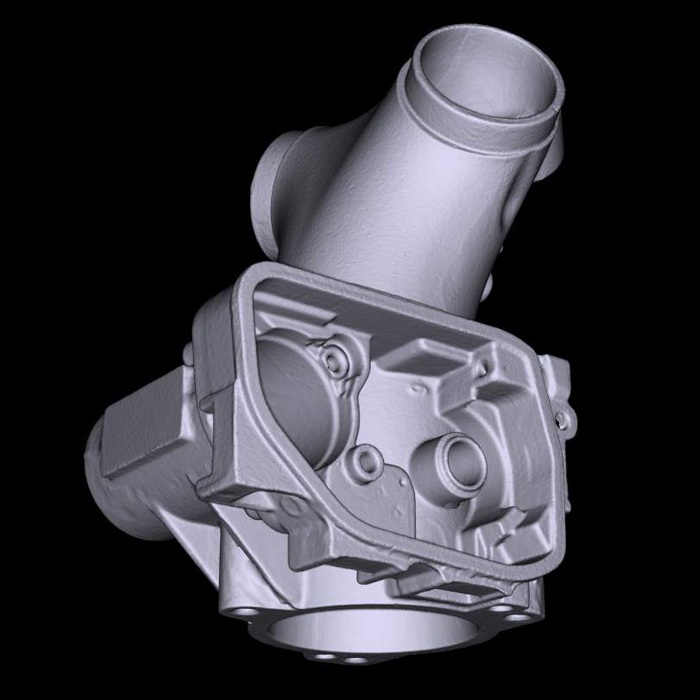
\includegraphics[width=0.49\linewidth]{images/lmi3d/throttle2}
        }
        \\
        \subfloat[Ingeniería inversa de piezas]
        {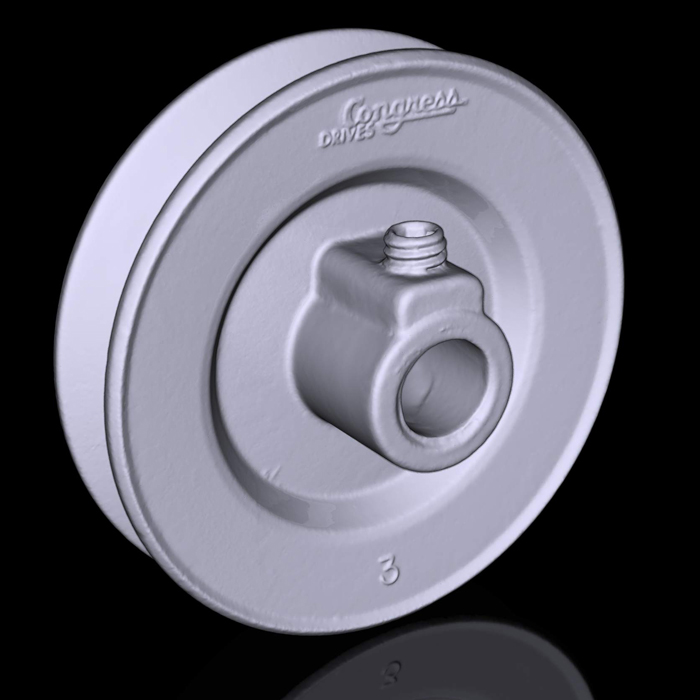
\includegraphics[width=0.49\linewidth]{images/lmi3d/pulley}
         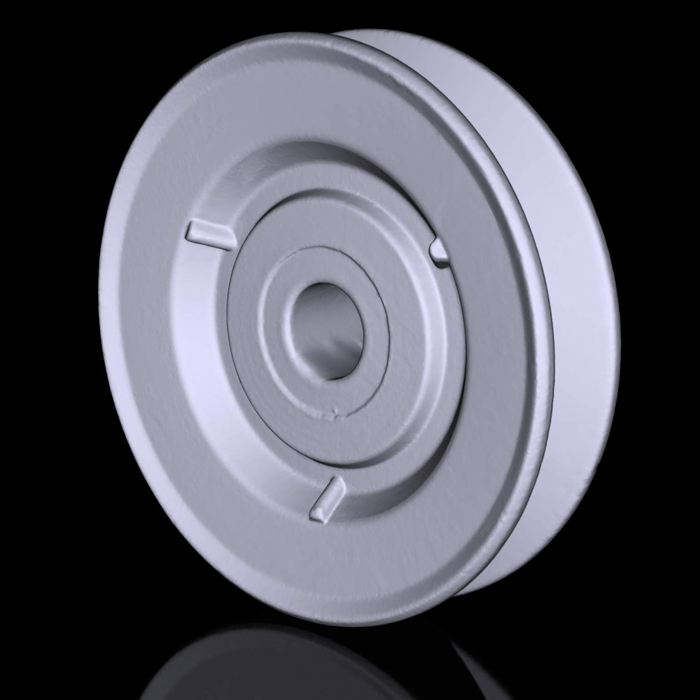
\includegraphics[width=0.49\linewidth]{images/lmi3d/pulley2}
        }
        \caption{Ejemplos de usos de metrología óptica (lmi3d.com)}
        \label{fig:metrologiaOpticaEjemplos1}
\end{figure}

\begin{figure}[!bth]
    \myfloatalign
        \subfloat[Odontología: digitalización de modelos dentales]
        {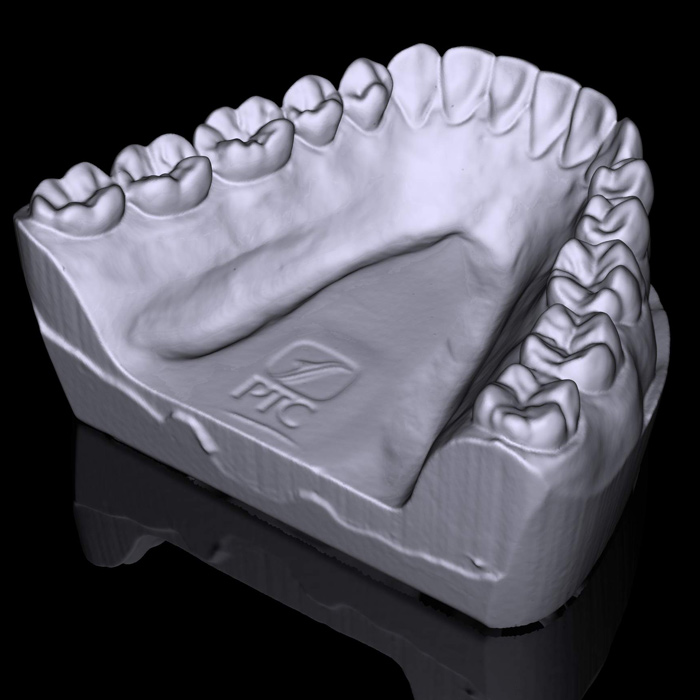
\includegraphics[width=0.49\linewidth]{images/lmi3d/dental-5mp}
         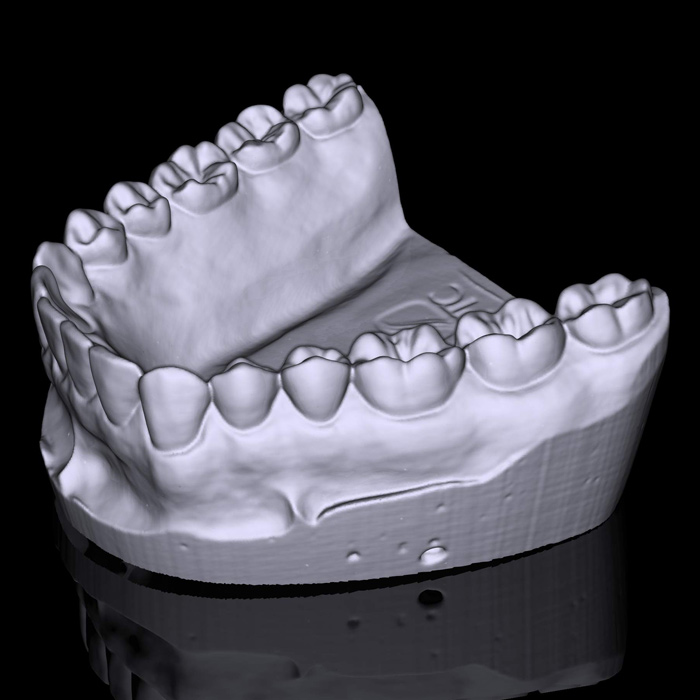
\includegraphics[width=0.49\linewidth]{images/lmi3d/dental-5mp2}
        }
        \\
        \subfloat[Medicina]
        {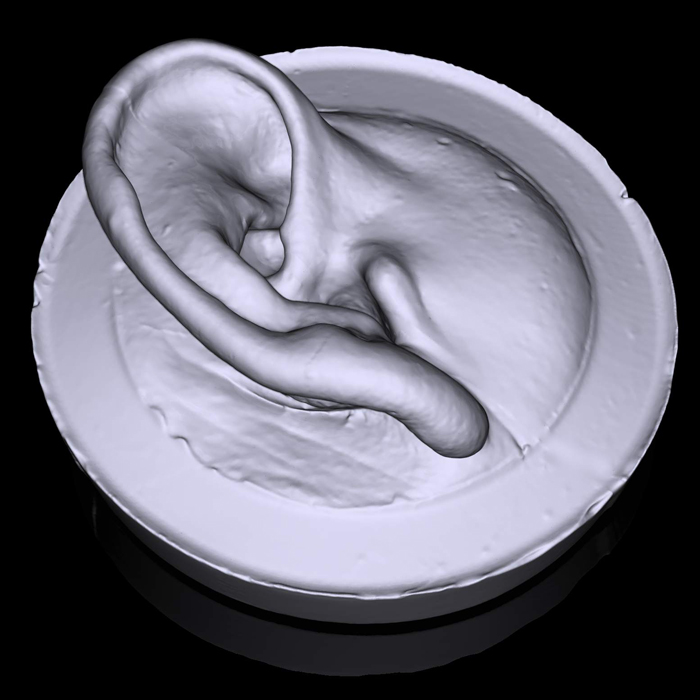
\includegraphics[width=0.49\linewidth]{images/lmi3d/ear-mold}
         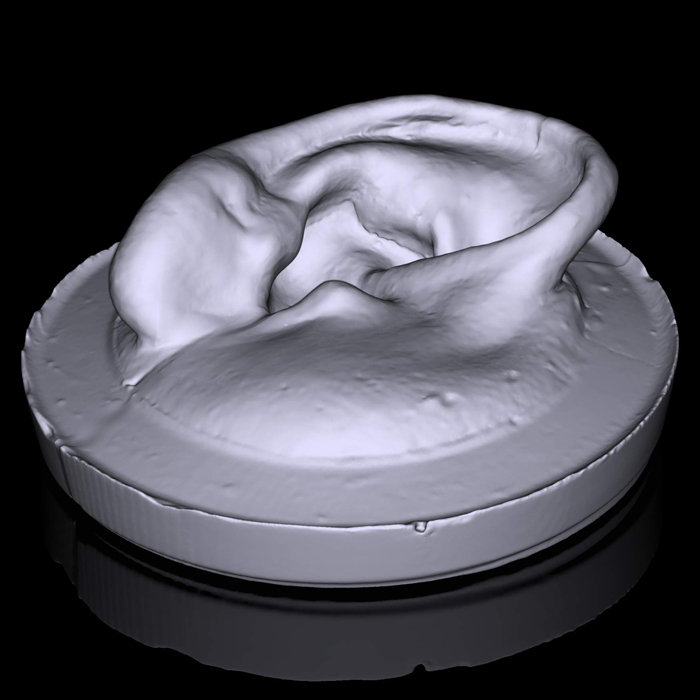
\includegraphics[width=0.49\linewidth]{images/lmi3d/ear-mold2}
        }
        \caption{Ejemplos de usos de metrología óptica (lmi3d.com)}
        \label{fig:metrologiaOpticaEjemplos2}
\end{figure}

\begin{figure}[!bth]
    \myfloatalign
        \subfloat[Conservación/digitalización de piezas artísticas]
        {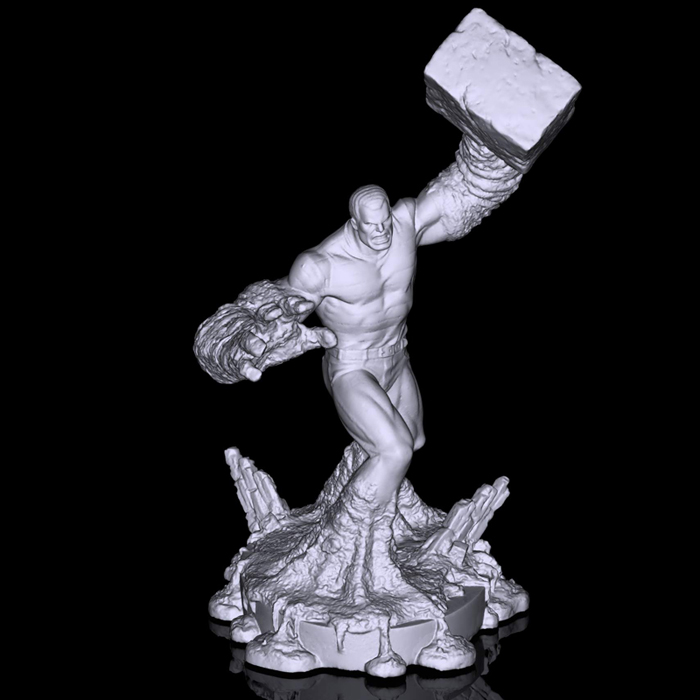
\includegraphics[width=0.49\linewidth]{images/lmi3d/sandman}
         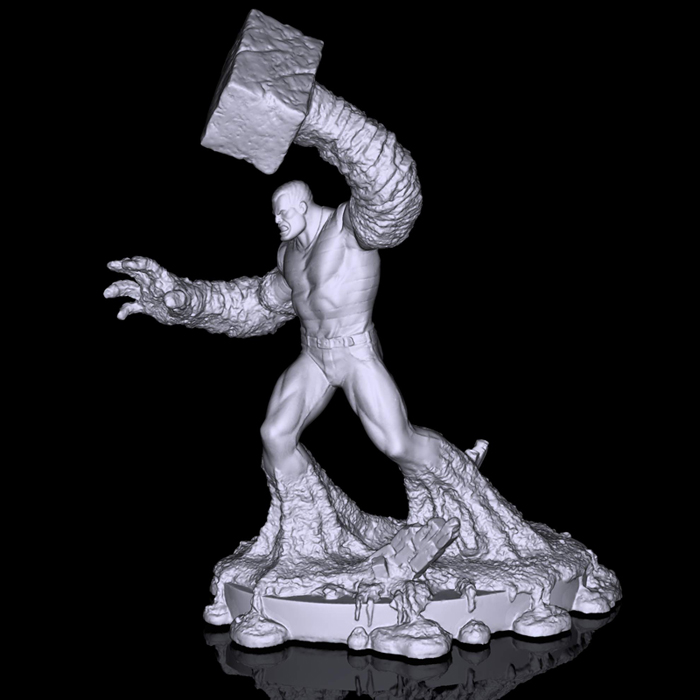
\includegraphics[width=0.49\linewidth]{images/lmi3d/sandman2}
        }
        \\
        \subfloat[Generación de modelos para la animación digital]
        {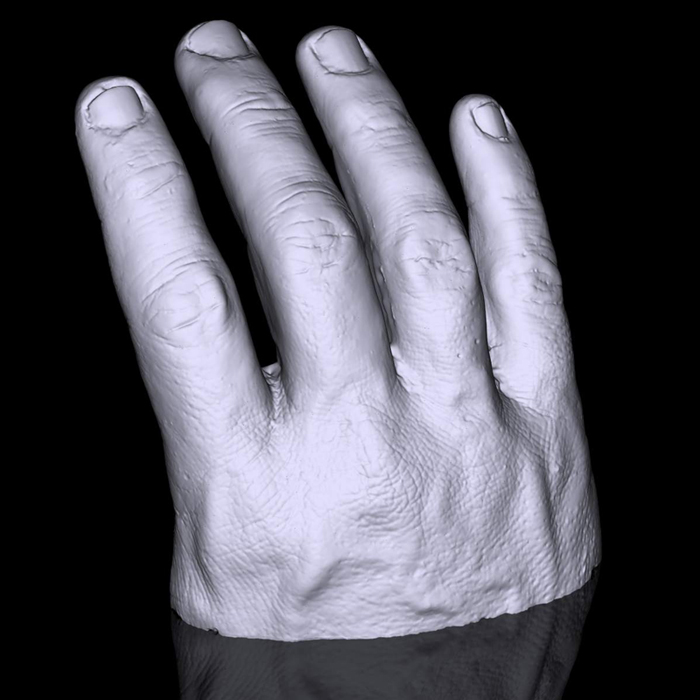
\includegraphics[width=0.49\linewidth]{images/lmi3d/hand-mold}
         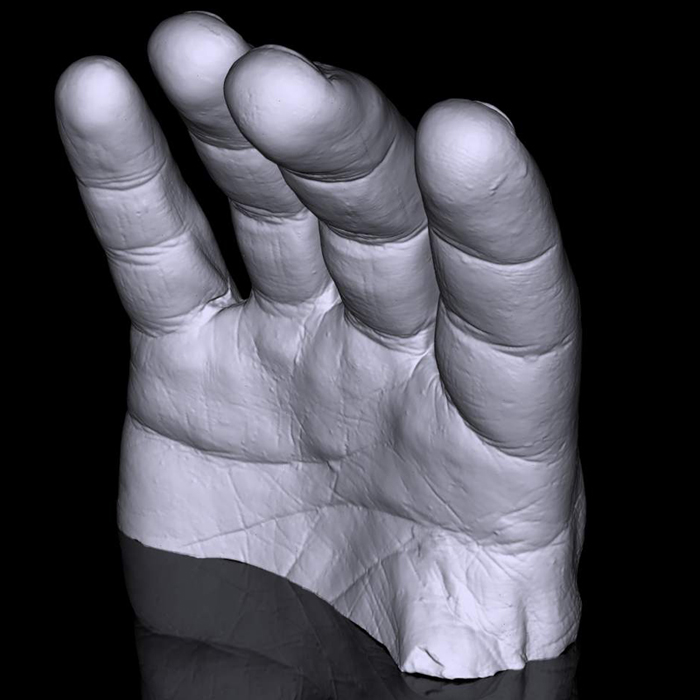
\includegraphics[width=0.49\linewidth]{images/lmi3d/hand-mold2}
        }
        \caption{Ejemplos de usos de metrología óptica (lmi3d.com)}
        \label{fig:metrologiaOpticaEjemplos3}
\end{figure}

Debido a su funcionamiento sin contacto, las técnicas de inspección óptica se presentan como una alternativa muy interesante para este tipo de aplicaciones. Si bien diversos métodos ópticos de medición son conocidos desde hace décadas, la evolución y abaratamiento experimentados en los últimos años en las computadoras, dispositivos de obtención de imágenes digitales, componentes electro-ópticos, láseres y otras fuentes de luz permitieron su aplicación con éxito en diversos ambientes industriales y de consumo masivo.

Existe una gran variedad de técnicas ópticas tridimensionales: triangulación láser, luz estructurada, visión estéreo, fotogrametría, tiempo de vuelo, interferometría, entre otras \cite{sansoni2009state}. Entre ellos se destacan los métodos de luz estructurada y triangulación láser debido a su bajo costo, robustez, flexibilidad, velocidad y principalmente su precisión y resolución \cite{gorthi2010fringe}. Estos métodos se utilizan con éxito para medir elementos a diferentes escalas, partiendo desde pequeños componentes \ac{MEMS} hasta grandes paneles de hasta 2 metros de largo, chequeo de la geometría de paneles de estampado, medición de deformaciones, análisis de corrosión, etc, existiendo diversas empresas que ofrecen dispositivos e incluso soluciones completas de manera comercial\footnote{\url{http://www.gom.com/metrology-systems/3d-scanner.html}}\footnote{\url{http://lmi3d.com/products/hdi/}}\footnote{\url{http://lmi3d.com/products/gocator/snapshot-sensor/}}\footnote{\url{http://geomagic.com/en/products/capture/overview/}}.

%\cite{wwwGOM},\cite{wwwLMI3Dhdi}, \cite{wwwLMI3Dsnapshotsensor}.

Los dispositivos disponibles comercialmente suelen ser relativamente fáciles de utilizar y muchas veces vienen calibrados desde fábrica, pero este mismo hecho limita su flexibilidad respecto al rango de medición y la distancia mínima de trabajo (comúnmente conocida como \emph{standoff}). Al tratarse de soluciones cerradas, se limitan considerablemente las posibilidades de adaptación para su uso en situaciones particulares. Como ejemplo, un producto\footnote{Cámara 3D Fotonic TOF-C70E, más detalles disponibles en \url{http://www.fotonic.com/assets/documents/products/Fotonic_C-series.pdf}} del cual se dispone actualmente en el laboratorio de Física Aplicada del Centro de Investigación Industrial de Tenaris Siderca, basado en tiempo de vuelo, no logra la precisión deseada (menor a $1$ mm) y tampoco resulta suficiente su resolución (genera una imagen en profundidad de $160x120$ pixels, lo que equivale a sólo $19200$ puntos, con una distancia mínima entre ellos de aproximadamente $4$mm).

En este proyecto se propone el desarrollo de un dispositivo de medición en tres dimensiones utilizando técnicas de metrología óptica, y evaluar su aplicación para la ubicación y el dimensionamiento de objetos cilíndricos en un ambiente industrial.

El desarrollo de un dispositivo a medida brindará la flexibilidad requerida para optimizar el balance entre precisión y rango de medición necesarios y permitirá obtener la resolución deseada. Otros beneficios importantes son el completo control sobre las diversas etapas de la reconstrucción de la geometría en tres dimensiones y la generación de una base tecnológica sólida sobre la cual continuar evolucionando la tecnología. Los desarrollos, el conocimiento y la experiencia adquiridos podrán ser utilizados luego como punto de partida para el desarrollo de nuevas soluciones a otros problemas similares.


\section{Objetivos}
\begin{itemize}
	\item Generales:
		\begin{itemize}
			\item Desarrollar un dispositivo para detectar la presencia de un 
			objeto cilíndrico en el espacio y determinar con precisión su 
			ubicación y dimensiones.
		\end{itemize}
	\item Específicos:
		\begin{itemize}
			\item Obtener conocimiento sobre técnicas y algoritmos de metrología
			 óptica, luz estructurada, triangulación.
			\item Adquirir conocimientos en los fundamentos de la óptica, la 
			fotografía digital y la geometría computacional aplicables a estos 
			métodos de medición.
			\item Desarrollar un método para facilitar la calibración del sistema.
			\item Estimar la precisión que se puede lograr bajo distintas 
			configuraciones del sistema.
		\end{itemize}
\end{itemize}

%En cuanto al resultado final, se busca que el dispositivo cumpla los siguientes objetivos:
%    \begin{itemize}
%        \item\texttt{rápido:} aunque el objeto bajo inspección se mantiene estacionario durante el proceso de medición, el dispositivo debe ser rápido para permitir que el objeto siga su curso dentro de la línea de producción.
%        \item\texttt{sin partes móviles:} el dispositivo no debe contener partes móviles para lograr mayor robustez, considerando su posible uso en un ambiente industrial.
%        \item\texttt{flexible:} se debe brindar la flexibilidad requerida para obtener el rango de medición, distancia de stand off, precisión, resolución y velocidad buscados.
%        \item\texttt{fácil de calibrar:} la flexibilidad debe ir acompañada de un procedimiento que permita calibrar fácilmente el dispositivo para cada configuración utilizada.
%    \end{itemize}




\section{Organización de la tesis}
En el primer capítulo se expone la motivación y los principales objetivos del proyecto.
En el segundo capítulo se realizará una introducción a los sistemas ópticos de medición con especial énfasis en los métodos basados en triangulación. En el tercer capítulo se explicará en detalle todo lo relacionado a la óptica del sistema y la calibración del principal componente, la cámara. En el cuarto capítulo se explican los detalles del prototipo desarrollado, tanto respecto al hardware como software. En el quinto capítulo se muestran algunos resultados obtenidos y finalmente la conclusiones se presentan en el sexto capítulo. 




\begin{figure}[!bth]
    \myfloatalign
        %\subfloat [Inspección en la industria automotriz]
        %{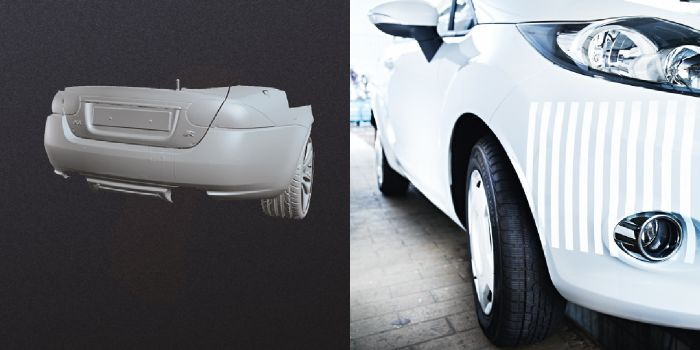
\includegraphics[width=1\linewidth]{images/david-3d.com/car}}
        %\\
        %\subfloat [Usos biométricos]
        %{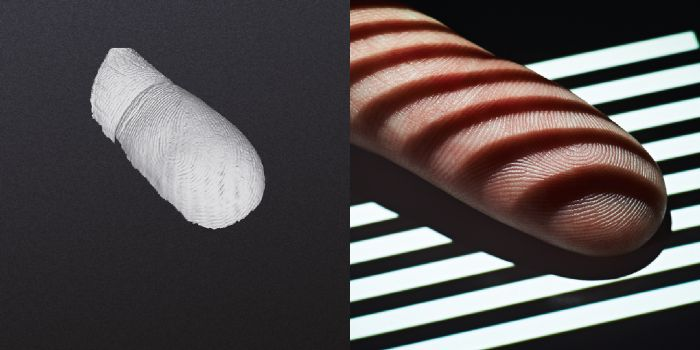
\includegraphics[width=1\linewidth]{images/david-3d.com/finger}}
        %\\
        \subfloat [Uso medicinal: corrección de la postura]
        {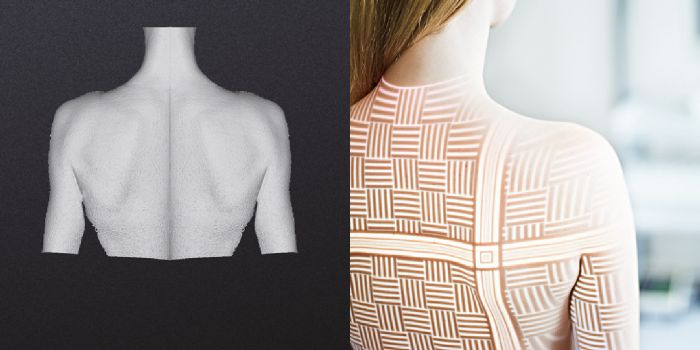
\includegraphics[width=1\linewidth]{images/david-3d.com/body}}
        \\
        \subfloat [Preservación de evidencias para uso forense]
        {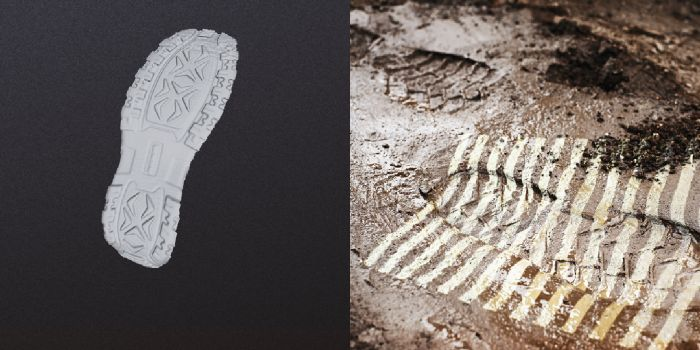
\includegraphics[width=1\linewidth]{images/david-3d.com/forensics}}
        \caption{Ejemplos de usos de metrología óptica (david-3d.com)}
        \label{fig:metrologiaOpticaEjemplos4}
\end{figure}

%*****************************************
%*****************************************
%*****************************************
%*****************************************
%*****************************************




